In der Messung werden für den Frequenzbereich von 6000 bis 9000 $\si{Hz}$ Rohrlängen von $\SI{75}{mm}$ bis $\SI{600}{mm}$ vermessen.
Bei bestimmten Frequenzen bildet sich eine stehende Welle aus. Das hat Resonanz zur Folge, so dass die Schallwelle eine höhere Intensität hat.
In den folgenden Abbildungen wird die Intensität gegen die Wellenlänge aufgetragen.
In der Abbildung \ref{fig.1} sind die Messwerte für die Rohrlängen: $\SI{75}{mm}, \SI{150}{mm}, \SI{225}{mm}, \SI{300}{mm}$ abbgebildet.
\begin{figure}[h!]
  \centering
  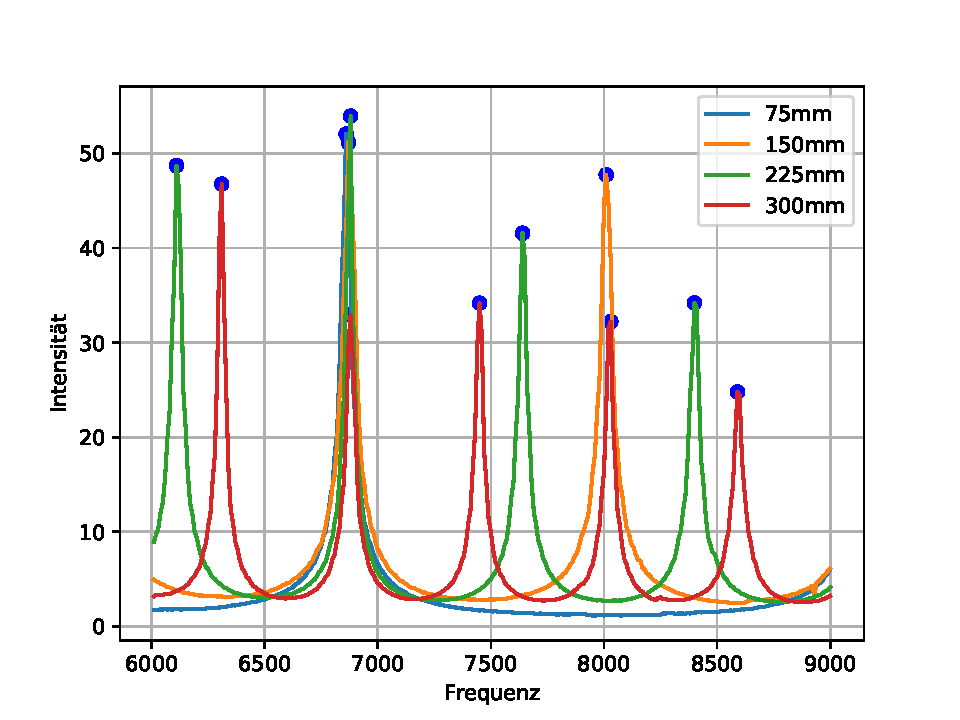
\includegraphics[width=\textwidth]{1234.pdf}
  \caption{Intensität der Schallwelle im Bereich von 6000 bis 9000 $\si{Hz}$ für die Rohrlängen $\SI{75}{mm}, \SI{150}{mm}, \SI{225}{mm}, \SI{300}{mm}$}
  \label{fig.1}
\end{figure}
In der Abbildung \ref{fig.2} sind die Messwerte für die Rohrlängen: $\SI{375}{mm}, \SI{450}{mm}, \SI{525}{mm}, \SI{600}{mm}$ dargestellt.
\begin{figure}[h!]
  \centering
  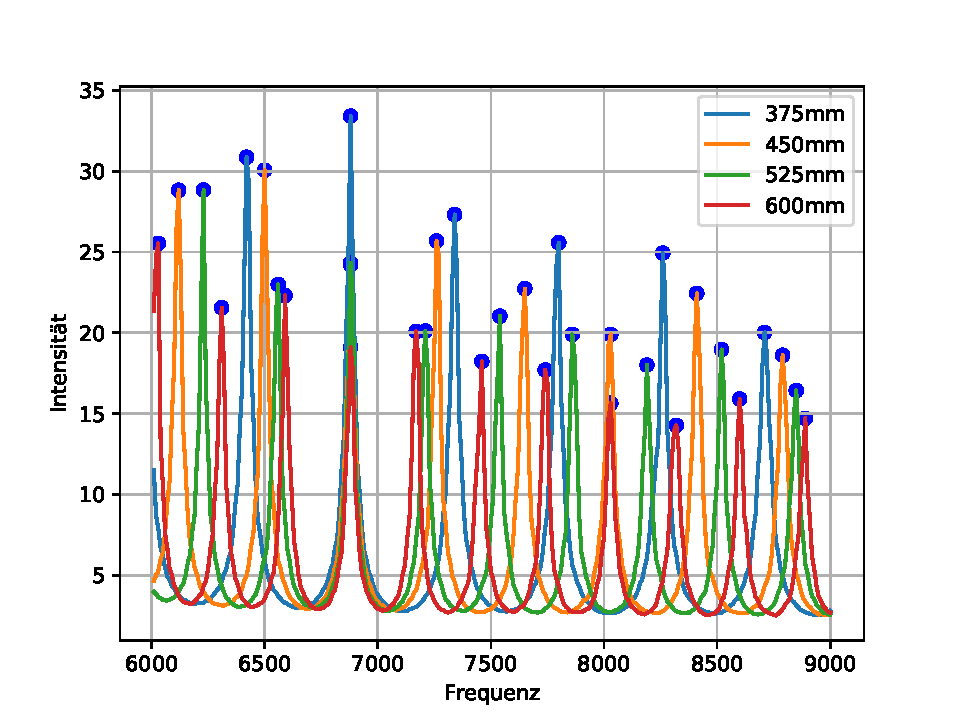
\includegraphics[width=\textwidth]{5678.pdf}
  \caption{Intensität der Schallwelle im Bereich von 6000 bis 9000 $\si{Hz}$ für die Rohrlängen $\SI{375}{mm}, \SI{450}{mm}, \SI{525}{mm}, \SI{600}{mm}$}
  \label{fig.2}
\end{figure}
Die Intensitätsmaxima sind mit einem blauen Punkt gekennzeichnet.
%Auffällig ist, dass sich für alle Rohrlängen Intensitätsmaxima an der Stelle von $\SI{6880}{Hz}$ bilden.
%Das heißt, dass bei dieser Frequenz eine stehende Welle entsteht die eine Wellenlänge von $\lambda=\frac{1}{2n}d$ besitzt.
%$d$ ist dabei die Länge des Rohres und n die Anzahl der Knotenpunkte.
%Desweiteren ist auffällig, dass für eine Rohrlänge der Abstand zwischen zwei Maxima immer konstant ist.
\FloatBarrier

\subsection{Aufgabe 1: Bestimmung der Schallgeschwindigkeit}
\FloatBarrier
In den Graphen \ref{fig.1} und \ref{fig.2} %\textbf{\huge{DAS IST ZWEI MAL DER GLEICHE PLOT (4\&4)}}
werden die Resonanzfrequenzen einer jeden Messreihe von 1 bis n nummeriert und anschließend gegen die Frequenz aufgetragen.
Die Resonanzfrequenzabstände sind konstant für eine Messreihe, daher ergeben sich Geraden der Form:
\begin{equation*}
  y=ax+b,
\end{equation*}
welche mit Python 3.6.3 und curve\_fit an die Messwerte gefittet werden.
Für die Besimmung der Steigung der Geraden ist die richtige Nummerierung der Resonanzfrequenzen nicht von bedeutung.
Es genügt wenn in einer Messung vortlaufend nummeriert wird.
In der Abb. \ref{fig.linearfit} sind die Messwerte mit den Fitfunktionen abgebildet.
%Für die Fitparameter ergeben sich folgende Werte.
%\begin{align*}
%  a &= 286.54545455 \pm 0.37848474\\
%  b &= 5737.09090907 \pm 2.56700835
%\end{align*}
Mit Hilfe der Steigung $a$ kann die Schallgeschwindigkeit $c$ berechnet werden.
\begin{align*}
  c = a\cdot2d
\end{align*}
Für die Schallgeschwindigkeit ergeben sich so Werte von:
\begin{table}
  \centering
  \caption{Bestimmung der Schallgeschwindigkeit}
  \label{Tab1}
    \begin{tabular}{c c c}
      \toprule
      Steigung&Rohrlänge&Schallgeschwindigkeit\\
      a&d&c\\
      \midrule
      $\si{\frac{1}{s}}$&$\si{m}$&$\si{\frac{m}{s}}$\\
      \midrule
      \midrule
       1140.0 & 2$\cdot\SI{0.075}{m}$ & $\SI{342.0}{\frac{m}{s}}$\\
       763.0  & 3$\cdot\SI{0.075}{m}$ & $\SI{343.3}{\frac{m}{s}}$\\
       571.0  & 4$\cdot\SI{0.075}{m}$ & $\SI{342.6}{\frac{m}{s}}$\\
       458.6  & 5$\cdot\SI{0.075}{m}$ & $\SI{343.9}{\frac{m}{s}}$\\
       381.9  & 6$\cdot\SI{0.075}{m}$ & $\SI{343.7}{\frac{m}{s}}$\\
       327.2  & 7$\cdot\SI{0.075}{m}$ & $\SI{343.5}{\frac{m}{s}}$\\
       286.5  & 8$\cdot\SI{0.075}{m}$ & $\SI{343.8}{\frac{m}{s}}$\\
      \bottomrule
    \end{tabular}
\end{table}
%\begin{align*}
%a &= 1140.0 && d = 2\cdot\SI{0.075}{m} && c=\SI{342.0}{\frac{m}{s}}\\
%a &= 763.0  && d = 3\cdot\SI{0.075}{m} && c=\SI{343.3}{\frac{m}{s}}\\
%a &= 571.0  && d = 4\cdot\SI{0.075}{m} && c=\SI{342.6}{\frac{m}{s}}\\
%a &= 458.6  && d = 5\cdot\SI{0.075}{m} && c=\SI{343.9}{\frac{m}{s}}\\
%a &= 381.9  && d = 6\cdot\SI{0.075}{m} && c=\SI{343.7}{\frac{m}{s}}\\
%a &= 327.2  && d = 7\cdot\SI{0.075}{m} && c=\SI{343.5}{\frac{m}{s}}\\
%a &= 286.5  && d = 8\cdot\SI{0.075}{m} && c=\SI{343.8}{\frac{m}{s}}\\
%\end{align*}
Der Mittelwert ergibt:
\begin{align*}
  c=\SI{343.28\pm1.63}{\frac{m}{s}}.
\end{align*}
%###########Bild##########
%\begin{figure}[h!]
%  \centering
%  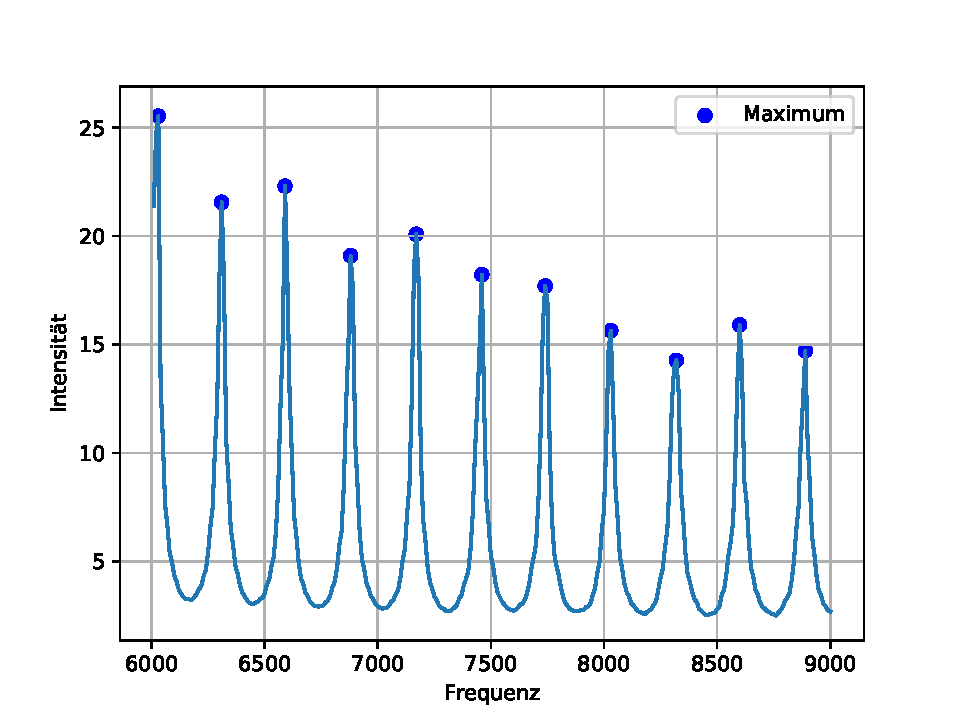
\includegraphics[width=\textwidth]{A1L8x75mmF6000-9000S10.pdf}
%  \caption{Messung eines $\SI{0.6}{m}$ Rohres für den Frequenzbereich von 6000 bis 9000 Hz}
%  \label{fig.frequenz/rohrlänge}
%\end{figure}
\begin{figure}[h!]
  \centering
  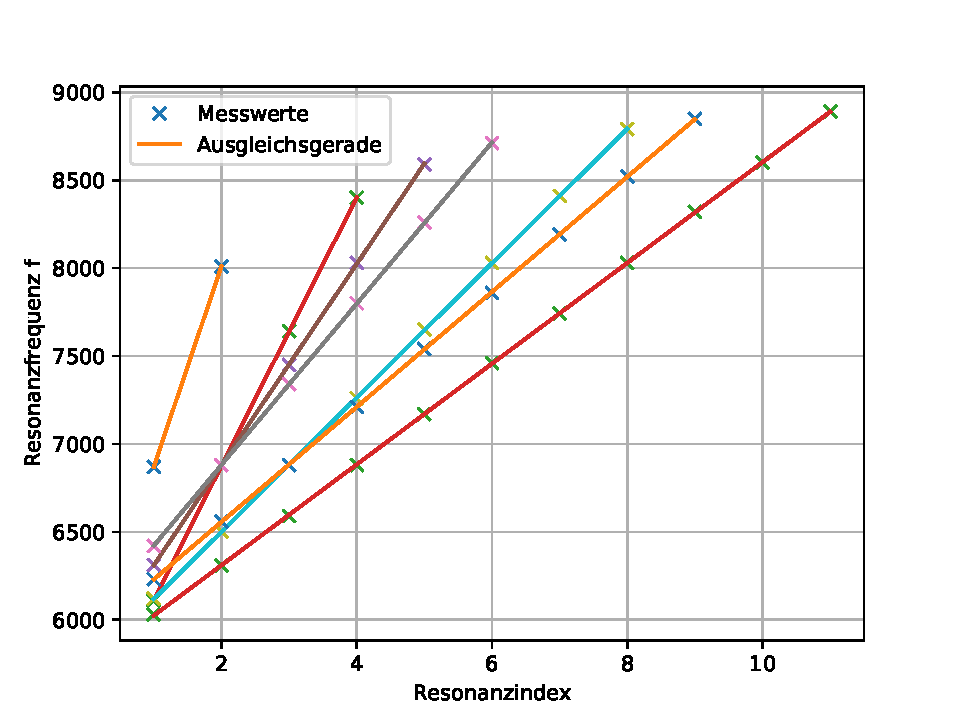
\includegraphics[width=\textwidth]{linearfit.pdf}
  \caption{Die Intensitätsmaxima werden nummeriert und die Nummer gegen die Frequenz aufgetragen.}
  \label{fig.linearfit}
\end{figure}
%#########
\FloatBarrier
Die Schallgeschwindigkeit kann auch mit Hilfe einer anderen Methode bestimmt werden.
Dazu betrachten wir ein Rohr der Länge $\SI{75}{mm}$ für die Frequenzen von 6000 bis 9000 $\si{Hz}$.
Da die Rohrlänge $d$ ein Vielfaches $n$ der halben Wellenlänge $\lambda$ ist gilt:
\begin{align*}
  \lambda = \frac{2d}{n}.
\end{align*}
Die Schallgeschwindigkeit ist gegeben durch:
\begin{equation*}
  c=f \cdot \lambda.
\end{equation*}
Daraus ergibt sich :
\begin{align*}
  n=1&&  c&=\SI{1032}{\frac{m}{s}}\\
  n=2&&  c&=\SI{516}{\frac{m}{s}}\\
  %\textbf{\huge{SOLL DAS SO IM TEXT AUSSEHEN? n und c rücken hier zusammen}} &&
\end{align*}
\begin{align}
  n=3&&  c&=\SI{344}{\frac{m}{s}}
  \label{eqn.schall}
\end{align}
\begin{align*}
  n=4&&  c&=\SI{258}{\frac{m}{s}}.
\end{align*}
Die Frequenz ist dabei gegeben als $\SI{6880}{\frac{m}{s}}$.
Diese Frequenz ist die einzige Frequenz im Frequenzbereich, welche bei allen Vielfachen der Rohrlänge von $\SI{75}{mm}$ vertreten ist,
zusehen ist dies in den Abb. \ref{fig.1} und \ref{fig.2}.
Den Ergebnissen aus \ref{eqn.schall} ist zu entnehmen, dass die Wellenlänge bei $\frac{3}{2}\lambda$ liegt, da die dazugehörige Schallgeschwindigkeit von $\SI{344}{\frac{m}{s}}$ gut zum den bereits berechneten Wert von $\SI{343.28}{\frac{m}{s}}$ passt.

\FloatBarrier
Desweiteren soll die Schallgeschwindigkeit mithilfe des Verhältnisses von Frequenzübergängen zu Rohrlänge bestimmt werden.
Dieser Zusammenhang ist in Abb. \ref{fig.1/x} dargestellt.
An die Messwerte wird eine Funktion der Form $a\cdot\frac{1}{x}+b$ gefittet.
Für a und b ergeben sich die Werte:
%\\\textbf{\huge{Katti?: Deine Einheit der Steigung a ist Hz*m.}}

\begin{align*}
  a&=\SI{168692.913\pm253.977}{Hz \cdot mm}\\
  b&=\SI{8.566\pm1.995}{Hz}.\\
\end{align*}
Durch umstellen der Gleichung \ref{eqn:dispersionschall} zu:
\begin{align*}
  nc=2Lf+b=2a+b
\end{align*}
ergibt sich für die Schallgeschwindigkeit ein Wert von: $c = \SI{345.95}{\frac{m}{s}}$
%################Bild#####################
\begin{figure}[h!]
  \centering
  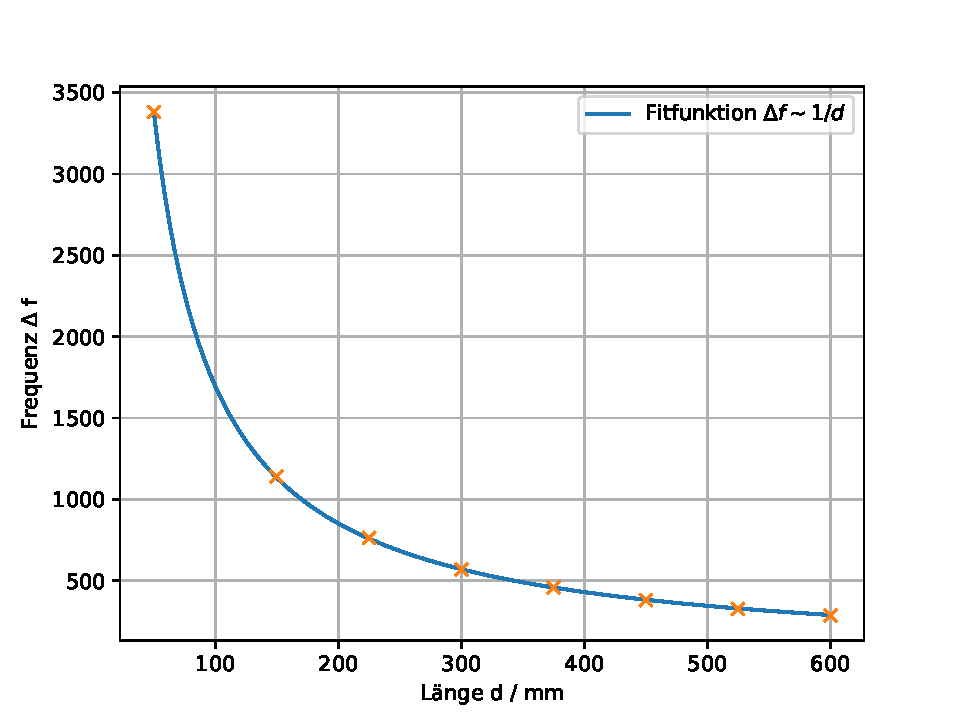
\includegraphics[width=\textwidth]{geschi.pdf}
  \caption{Der Abstand der Frequenzen wird gegen die Rohrlänge aufgetragen.}
  \label{fig.1/x}
\end{figure}
\FloatBarrier

\subsection{Aufgabe 2: Dispersion}
\FloatBarrier
In dieser Aufgabe soll als Grundlage zu den späteren Versuchsteilen gezeigt werden, wie die Dispersionsrelation $f(k)$ des akustischen Aufbaus im Gegensatz zur Dispersionsrelation des quantenmechanischen Teilchens im Potenzialtopf verläuft.
%In dieser Aufgabe wird $f(k)$ geplottet.
Aus der Messung mit einer Rohrlänge von $12\cdot\SI{50}{mm}$ und einem Frequenzbereich von $400-12000\si{Hz}$ werden die Maximalstellen mit Hilfe einer Peak-Picking-Funktion ermittelt.
Die Maximalstellen werden nummeriert und die dazugehörige Frequenz in $f(k)$ umgerechnet.
\begin{align}
  k= \frac{n \pi}{L}
\end{align}
$L$ ist dabei die gesammte Rohrlänge.

In der Abbildung \ref{fig.Aufgabe2} ist $k$ gegen $f(k)$ aufgetragen. Dargestellt ist zum einen die Dispersionsrelation von Schallwellen und zum anderen die Dispersionsrelation eines quantenmechanischen Teilchens im Potenzialtopf nach der Funktion \ref{eqn:dispersionqm}.
Es ist zu erkennen, dass die Dispersion von Schallwellen linear verläuft, wohingegen die Dispersion eines quantenmechanischen Teilchens im Potenzialtopf quadratisch ist.
%\textbf{\huge{DEN FOLGENDEN SATZ WÜRDE ICH NICHT IN DER AUSWERTUNG SCHREIBEN, SONDERN IN DER DISKUSSION, UND SELBST DA FINDE ICH IHN FRAGWÜRDIG. IMMERHIN HABEN WIR EINEN GANZEN VERSUCH DAMIT GEMACHT.}}
%Das Analogon zwischen den beiden Dispersionsrelationen ist daher nicht sehr zutreffend.
Aus der linearen Dispersion der Schallwelle folgt, dass wenn für ein kleines Rohr die Resonanzbedingung erfüllt ist gilt dies auch für vielfache der Rohrlänge.
Auf diese Weise lassen sich die Eigenheiten der Abbildungen \ref{fig.1} und \ref{fig.2} erklären.
\begin{figure}[h!]
  \centering
  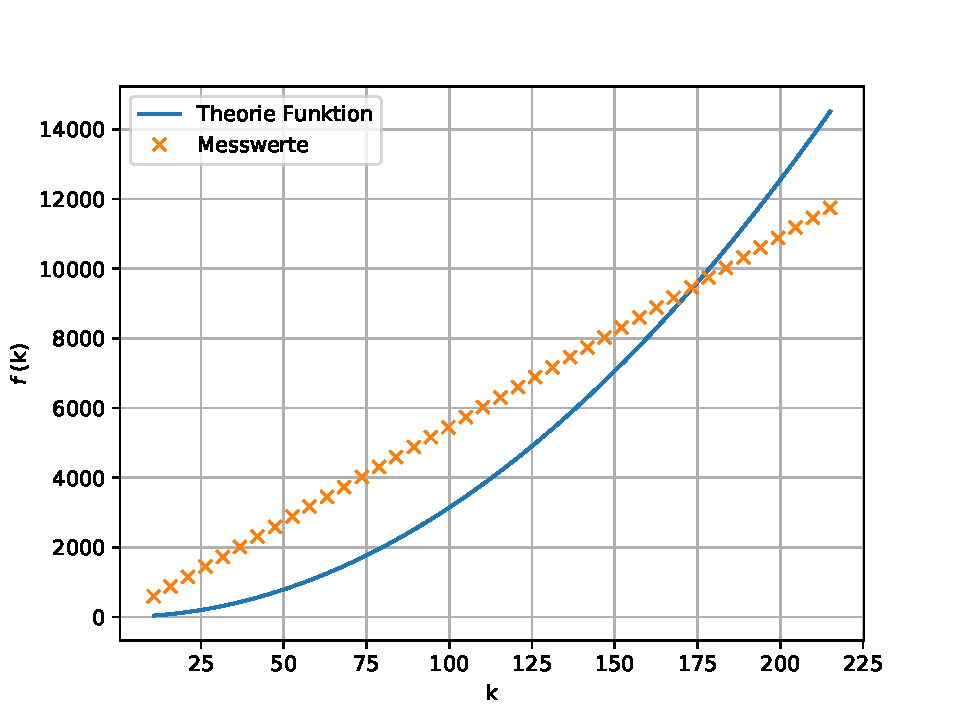
\includegraphics[width=\textwidth]{f(k).pdf}
  \caption{Dispersionsrelation für Schallwellen und die Theorie Funktion eines quantenmechanischen Teilchens im Potenzialtopf}
  \label{fig.Aufgabe2}
\end{figure}
%\textbf{\huge{Hat k im Plot keine Einheit? Ich weiß es so grade nicht :)}}
\FloatBarrier

\subsection{Aufgabe 3: Bandstrukturen}
\FloatBarrier
In dieser Aufgabe werden Atome in einer Kette simuliert um Bandlücken in dem akustischen System zu veranschaulichen.
Dazu wird ein Rohr der Länge $12 \cdot \SI{50}{mm}$ mit einheitlichen Blenden unterteilt.
Die Blendengrößen werden zwischen 10, 13 und $\SI{16}{mm}$ variiert.
In der Abbildung \ref{fig.Aufgabe3} werden die Bandlücken in Relation zu der Blendengröße dargestellt.
Für alle drei Messung mit den drei Blenden bilden sich drei Bandlücken aus, diese sind in der Abbildung jeweils übereinander.
Die untere Gerade stellt den Verlauf der ersten Bandlücke dar, die mittlere den Verlauf der zweiten Bandlücke und die obere den Verlauf der dritten Bandlücke.
Die zueinander gehörenden Bandlücken der unterschiedlichen Messungen sind jeweils mit einer Ausgleichsgeraden verbunden.
Es wird deutlich, dass die Bandlücken mit zunehmender Blendengröße kleiner werden.
Anders beschrieben wird die Kopplung zwischen einzelnen Rohren mir zunehmender Blendengröße größer wodurch sich das Spektrum einem Spektrum ohne Blenden annähert.
Die Bandlücken werden bestimmt, indem die Differenz vom Anfangs- und Endpunkt der Bandlücke betrachtet wird.
Die Bandlücken bei höherer Frequenz sind größer.
\begin{figure}[h!]
  \centering
  \includegraphics[width=\textwidth]{Bandlücken3.pdf}
  \caption{Größe der Bandlücken aufgetragen gegen die Blendengröße. Übereinander stehen jeweils die Messwerte einer Messung. Die zusammengehörigen Bandlücken werden über alle drei Messungen miteinander verbunden.}
  \label{fig.Aufgabe3}
\end{figure}
%\textbf{\huge{In den Achsenbeschriftungen ist an y 'Breite' falsch geschrieben, und an x 'Blendenbreite' - zieht sich so durch alle Plots}}
\FloatBarrier

\subsection{Aufgabe 4: Bandstrukturen}
In dieser Aufgabe und der folgenden geht es um die Vermessung der Einheitszellen des Systems.
Zunächst wird der Zusammenhang der Bandlücken und der Größe der gesamten Rohrlänge untersucht.
Hier werden wie bei der vorherigen Aufgabe die Bandlücken betrachet, jedoch im Verhältnis zur Rohrlänge statt zur Blendengröße.
Dementsprechend sind in der Abbildung \ref{fig.Aufgabe4} die Bandlücken gegen die Rohrlängen aufgetragen.
Die Rohrlänge wird zwischen $8 \cdot \SI{50}{mm}$, $10 \cdot \SI{50}{mm}$ und $12 \cdot \SI{50}{mm}$ variiert.
Wieder beschreibt die untere Gerade den Verlauf der ersten Bandlücke, die mittlere den Verlauf der zweiten Bandlücke und die obere den Verlauf der dritten Bandlücke.
Es ist zu erkennen, dass die Bandlücken unabhängig von der gesamten Rohrlänge sind.
Im übertragendem Sinn hängt die Bandlückenbreite nicht von der Größe des Kristalls ab.
\begin{figure}[h!]
  \centering
  \includegraphics[width=\textwidth]{Bandlücken.pdf}
  \caption{Größe der Bandlücken aufgetragen gegen die Rohrlänge. Übereinander stehen jeweils die Messwerte einer Messung. Die zusammengehörigen Bandlücken werden über alle drei Messungen miteinander verbunden.}
  \label{fig.Aufgabe4}
\end{figure}
\FloatBarrier

\subsection{Aufgabe 5}
In dieser Aufgabe wird der Zusammenhang der Bandlücken und der Größe der Einheitszellen gesetzt.
Dabei wird zwischen $8 \cdot \SI{75}{mm}$ und $8 \cdot \SI{50}{mm}$ gewechselt.
%Es werden dementsprechend unterschiedlich große Einheitszellen betrachtet.
In den Abbildungen \ref{fig.Aufgabe5} und \ref{fig.Aufgabe575} sind die Maxima gegen $k$ geplottet. Anhand der hinterlegten Bandlücken wird deutlich, dass die Bandlücken für größere Rohrabschnitte kleiner werden.
%In der Abbildung \ref{fig.Aufgabe5a} wird ebenfalls deutlich, dass die Größe der Bandlücke mit größeren Einheitszellen abfällt.
%\FloatBarrier

\begin{figure}
 \centering
 \begin{subfigure}{0.48\textwidth}
  \centering
  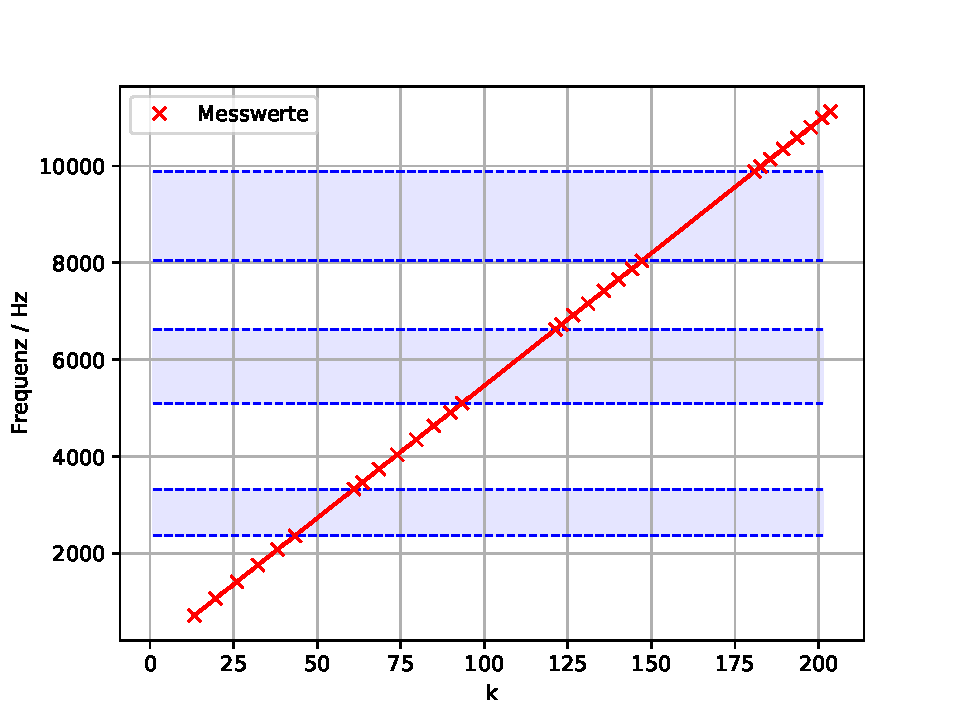
\includegraphics[width=1\textwidth]{bla.pdf}
  \caption{8 \cdot \SI{50}{mm}}
  \label{fig.Aufgabe5}
 \end{subfigure}
 \begin{subfigure}{0.48\textwidth}
  \centering
  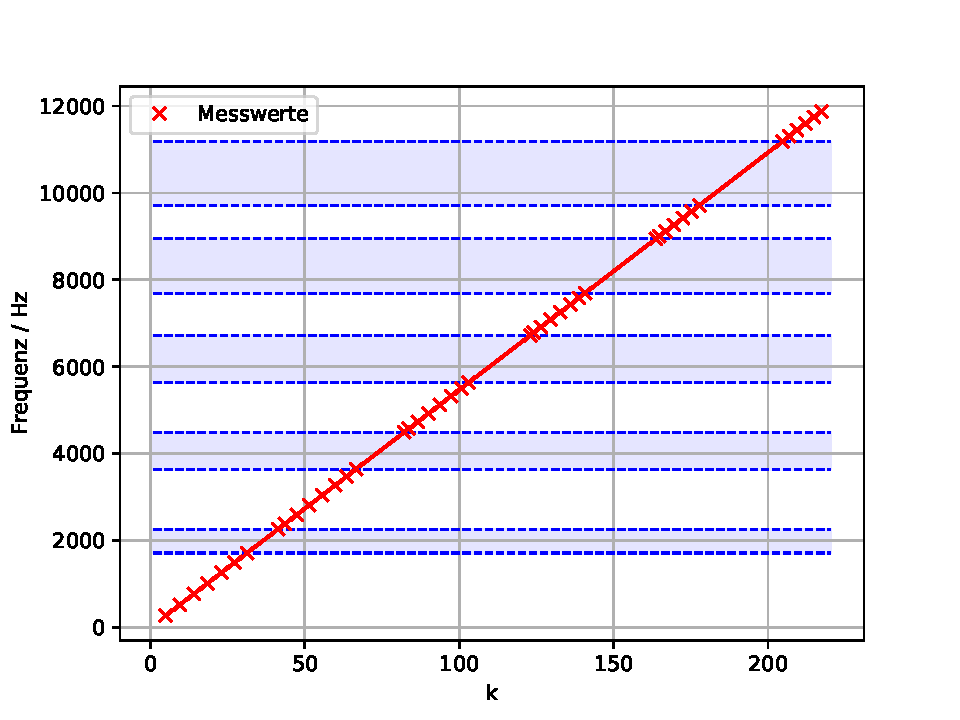
\includegraphics[width=1\textwidth]{bla75.pdf}
  \caption{8 \cdot \SI{75}{mm}}
  \label{fig.Aufgabe575}
 \end{subfigure}
 \caption{Bandlücken für unterschiedliche Rohrlängen}
 %\label{fig:500-6-7}
\end{figure}
%\textbf{\huge{Die beiden "Mini"-Plots haben an der x-Achse keine Einheit}}

\begin{figure}
 \centering
 \begin{subfigure}{0.48\textwidth}
  \centering
  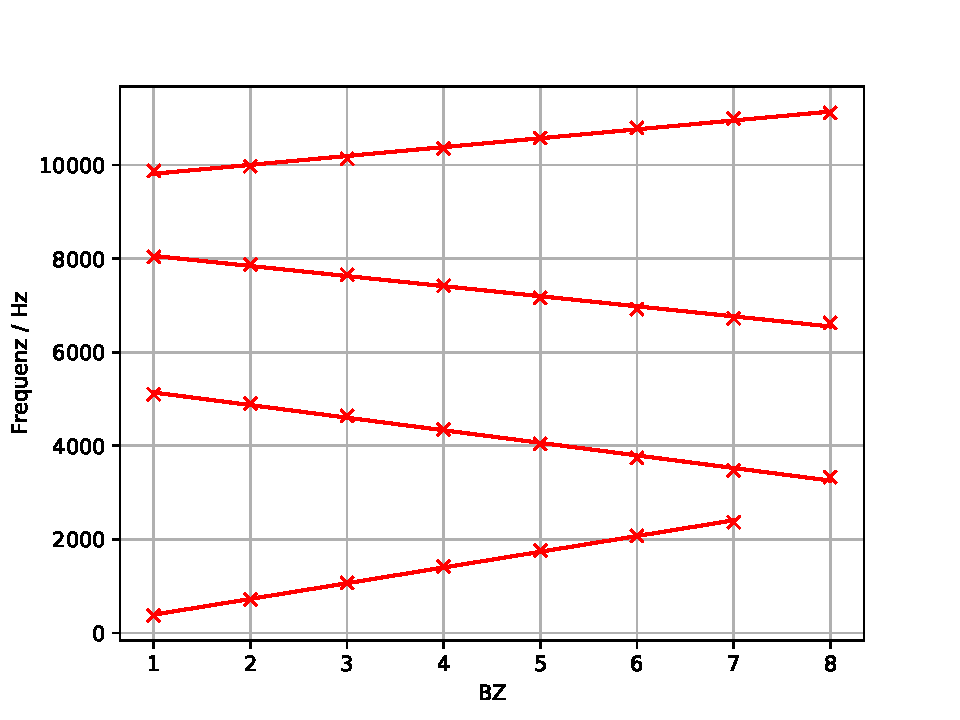
\includegraphics[width=1\textwidth]{RedBandSchem.pdf}
  \caption{8 \cdot \SI{50}{mm}}
  \label{fig.RedBandSchem}
 \end{subfigure}
 \begin{subfigure}{0.48\textwidth}
  \centering
  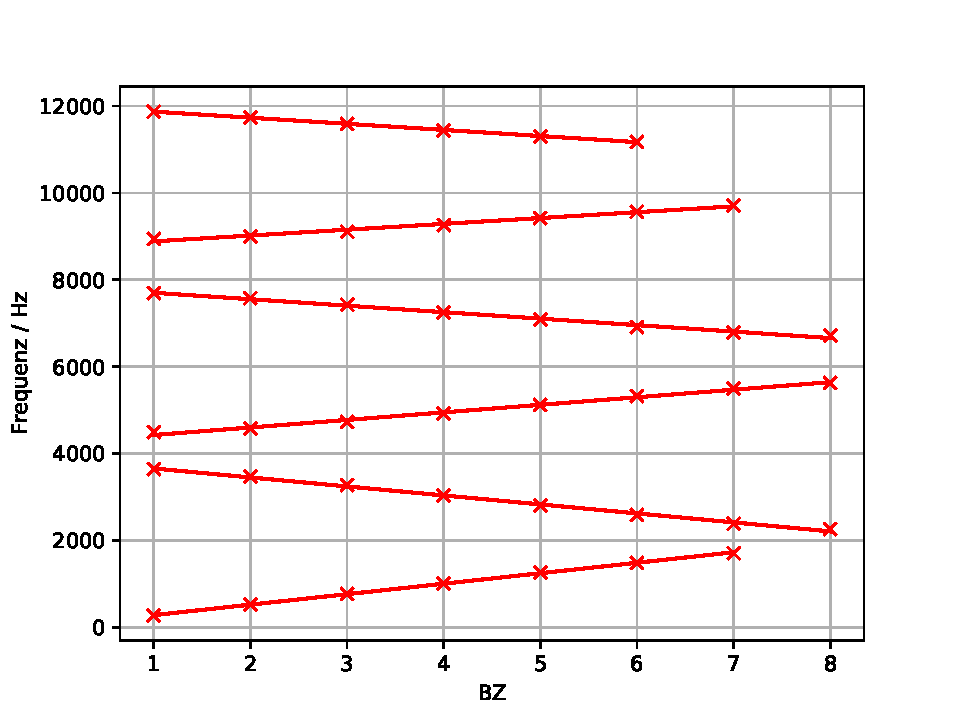
\includegraphics[width=1\textwidth]{RedBandSchem75.pdf}
  \caption{8 \cdot \SI{75}{mm}}
  \label{fig.RedBandSchem75}
 \end{subfigure}
 \caption{Reduziertes Bandlücken Schema}
 %\label{fig:500-6-7}
\end{figure}

In den Abbildungen \ref{fig.RedBandSchem} und \ref{fig.RedBandSchem75} werden dei Abbildungen \ref{fig.Aufgabe5} und \ref{fig.Aufgabe575} als reduziertes Bandschema dargestellt.
Die Darstellung im reduzierten Bandschema hat den Vorteil, dass die erlaubten Übergänge für Energie und Impuls senkrecht übereinander liegen.
Anhand der Abbildung \ref{fig.Aufgabe5} wird die Zustandsdichte mit Hilfe der Formel \ref{eqn:zustandsdichte} berechnet.
Die Zustandsdichte wird aus dem reziproken Frequenzabstand bestimmt.
Es ergibt sich für die Zustandsdichte ein Wert von:
\begin{equation*}
  \textbf{\huge{HIER}}.
\end{equation*}

%\begin{figure}[h!]
%  \centering
%  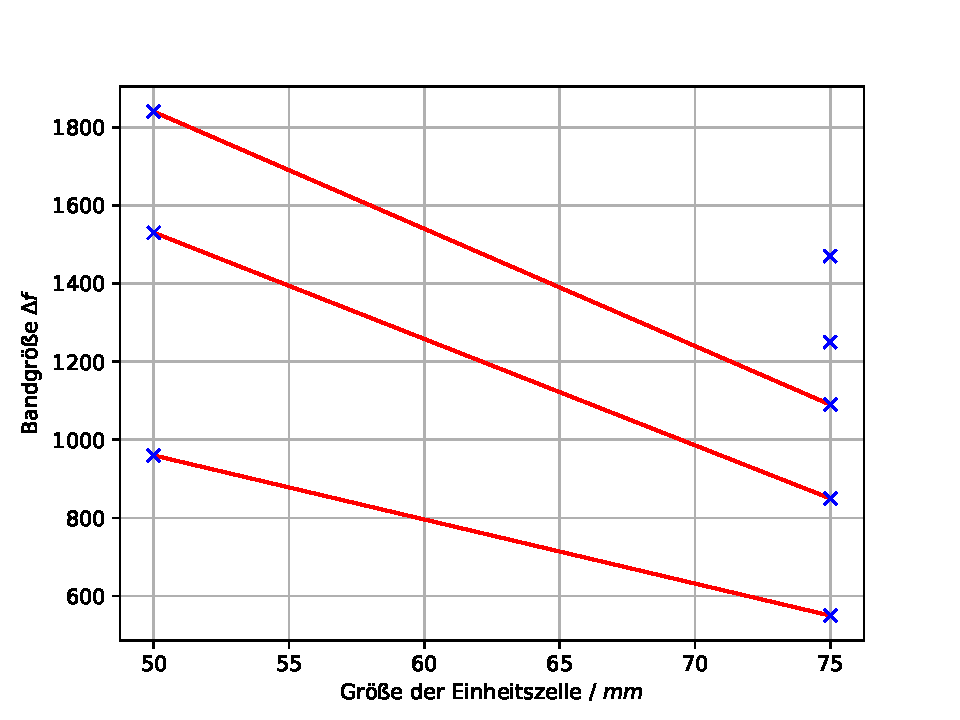
\includegraphics[width=\textwidth]{newtest.pdf}
%  \caption{Größe der Bandlücken aufgetragen gegen die Gesamtrohrlänge}
%  \label{fig.Aufgabe5a}
%\end{figure}
%\FloatBarrier
%
%\textbf{\huge{\ref{fig.Aufgabe5a} sieht irgendwie nicht sinnvoll aus, die Gerade sind nicht wirklich aussagekräftig, die einzige Aussage bekommen wir ja aus der kleineren Bandlückengröße bei größeren Röhrchen und das können wir oben bei den "Mini"-Plots schon gut erkennen..., außerdem ist die Achsenbeschriftung falsch. In dieser Aufgabe werden noch KEINE Einheitszellen betrachtet, war ne doofe Formulierung von mir mit den Zellen. }}

\FloatBarrier

\subsection{Aufgabe 6 und 7}
Nun wird eine Molekülkette behandelt.
Als Grundlage für die nächsten Aufgaben werden zwei einzelne Röhren vermessen und verglichen.
In dieser Aufgabe werden wieder die Maxima gegen k geplottet. Es entsteht wie erwartet eine Gerade welche in Abbildung \ref{fig.Aufgabe6} und \ref{fig.Aufgabe7} zu sehen ist.
Anhand der Abbildungen ist zu sagen, dass sich die beiden Messungen nicht viel unterscheiden.

\begin{figure}
 \centering
 \begin{subfigure}{0.48\textwidth}
  \centering
  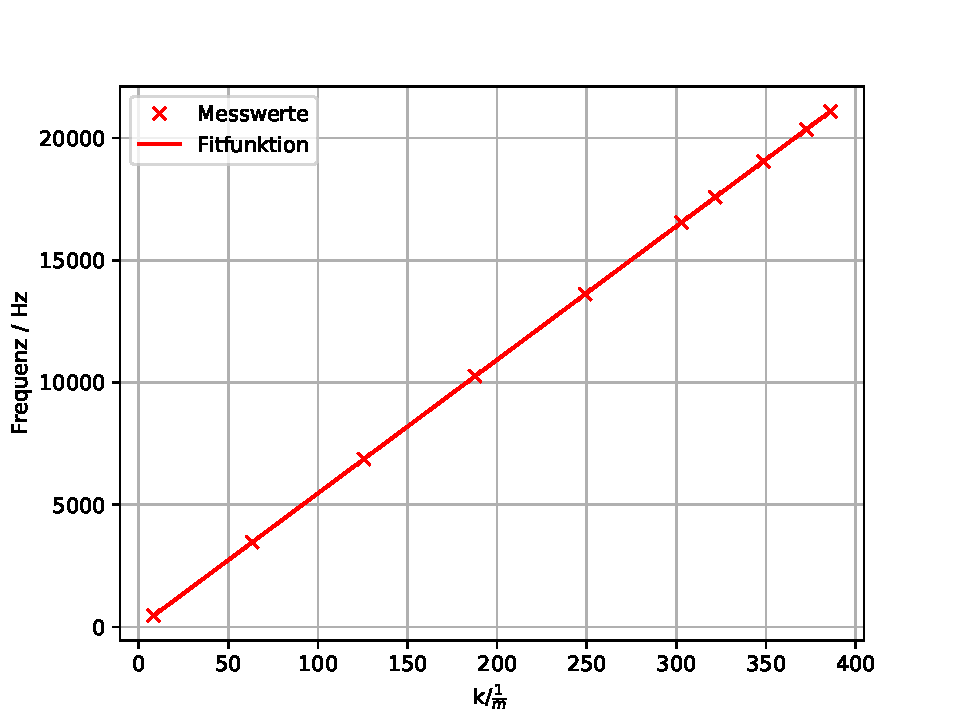
\includegraphics[width=1\textwidth]{A6.pdf}
  \caption{1 mal \SI{50}{mm}}
  \label{fig.Aufgabe6}
 \end{subfigure}
 \begin{subfigure}{0.48\textwidth}
  \centering
  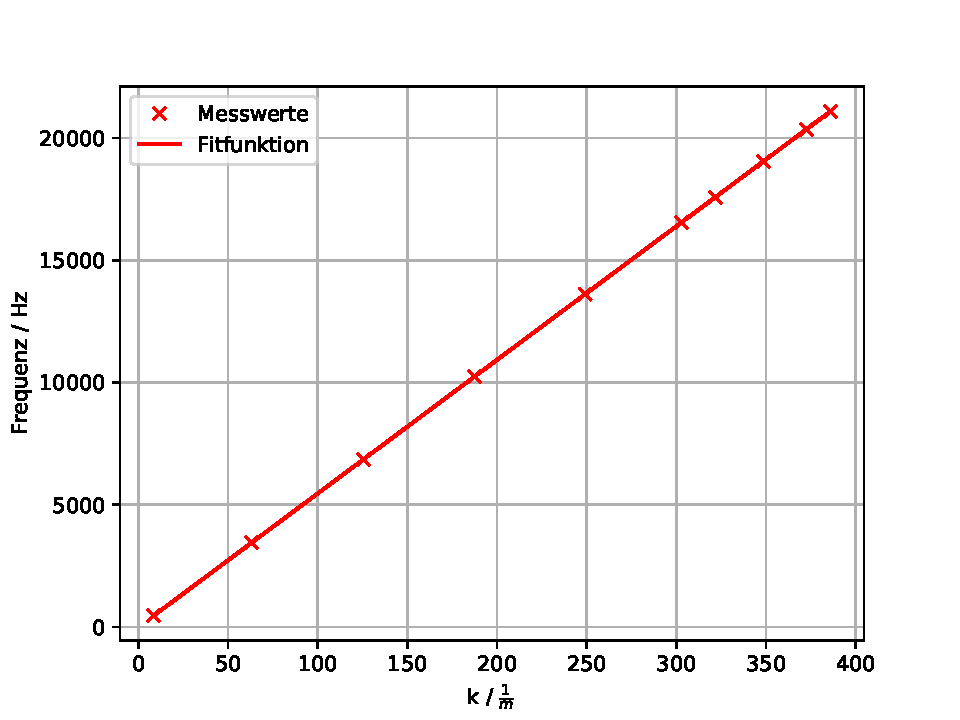
\includegraphics[width=1\textwidth]{A7.pdf}
  \caption{1 mal \SI{75}{mm}}
  \label{fig.Aufgabe7}
 \end{subfigure}
 \caption{Maxima gegen k}
 %\label{fig:500-6-7}
\end{figure}
%\textbf{\huge{Die Plots haben an der x-Achse keine Einheit}}
\FloatBarrier

\subsection{Aufgabe 8}
Die Molekülkette besteht nun aus einem Atom.
Es wird die Struktur der Bandlücken im Verhältnis zur Bindungsstärke der Atome untersucht.
Es werden für $2 \cdot \SI{50}{mm}$ Rohrlänge unterschiedliche Blendendurchmesser untersucht. Der Blendendurchmesser soll die Stärke der Bindungen zwischen den Atomen symbolisieren.
Für die unterschiedlichen Blendendurchmesser entstehen unterschiedlich breite Bandlücken.
In der Abbidung $\ref{fig.Aufgabe8}$ ist der Zusammenhang zwischen Blendendurchmesser und Bandlücke dargestellt.
Es wird deutlich, dass bei größeren Blendendurchmessern die Bandlücken kleiner werden.
\begin{figure}[h!]
  \centering
  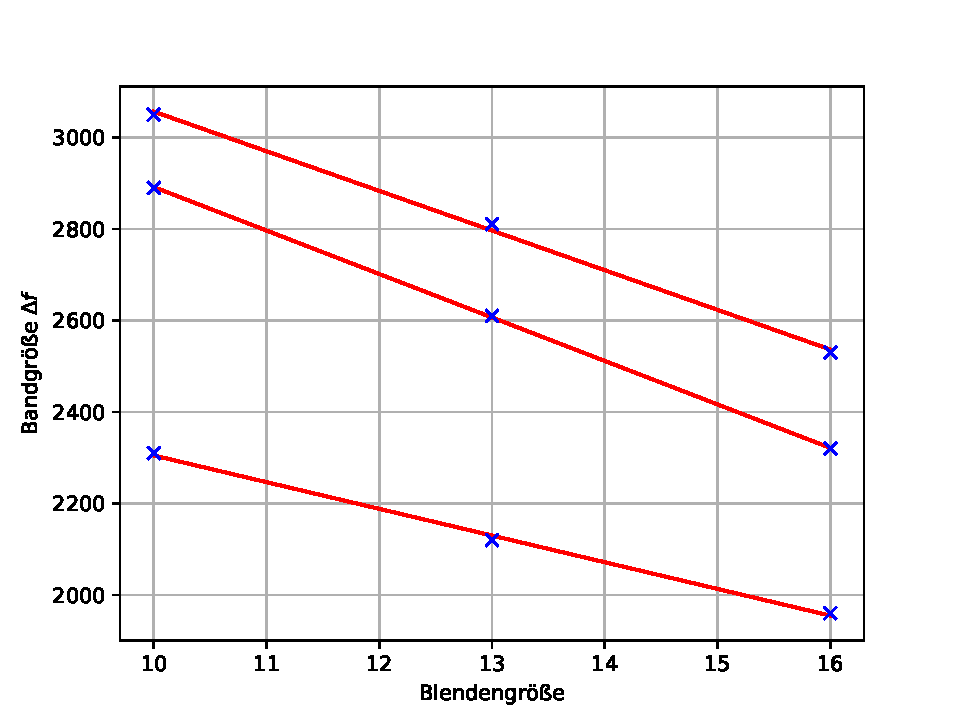
\includegraphics[width=\textwidth]{A8.pdf}
  \caption{Bandlücke in Abhängigkeit von dem Blendendurchmesser}
  \label{fig.Aufgabe8}
\end{figure}
\FloatBarrier

\subsection{Aufgabe 9}
In dem Aufgabenteil werden die Bandlücken in Abhängigkeit der Bindungsstärke und der Anzahl der Einheitszellen dargestellt.
Für die Blendengrößen von 10, 13 und 16 $\si{mm}$ werden jeweils 3, 4 und 6 Einheitszellen vermessen.
Die gemessenen Abhängigkeiten sind in den Abbildungen \ref{fig.Aufgabe9}, \ref{fig.Aufgabe91} und \ref{fig.Aufgabe92} abgebildet.
%Aus den Abbildungen wird deutlich, dass die Bandlückengröße mit steigender Anzahl von Einheitszellen linear ansteigt.
Die Bandlückenbreite bleibt mit steigender Zahl von Einheitszellen im wesentlichen konstant.
  \begin{figure}
   \centering
   \begin{subfigure}{0.48\textwidth}
    \centering
    \includegraphics[width=1\textwidth]{BandlückenD10.pdf}
    \caption{Blendendurchmesser $D=\SI{10}{mm}$}
    \label{fig.Aufgabe9}
   \end{subfigure}
   \begin{subfigure}{0.48\textwidth}
    \centering
    \includegraphics[width=1\textwidth]{BandlückenD13.pdf}
    \caption{Blendendurchmesser $D=\SI{13}{mm}$}
    \label{fig.Aufgabe91}
   \end{subfigure}
   \caption{Die Bandbreit in Abhängigkeit von der Anzahl der Einheitszellen}
   %\label{fig:500-6-7}
  \end{figure}
  \begin{figure}[h!]
    \centering
    \includegraphics[width=\textwidth]{BandlückenD16.pdf}
    \caption{Blendendurchmesser $D=\SI{16}{mm}$ in Abhängigkeit von der Anzahl der Einheitszellen}
    \label{fig.Aufgabe92}
  \end{figure}
  \FloatBarrier

\subsection{Aufgabe 10}
In diesem Aufgabenteil werden die Auswirkungen von periodischen Defekten auf die Bandlücken einer Molekülkette betrachtet.
Vermessen wird ein Rohr der Länge $L=12 \cdot \SI{50}{mm}$ mit abwechselnden Blendengrößen von 16 und 13 $\si{mm}$.
Die Frequenz der Maxima wird gegen k geplottet und die Bandlücken farbig makiert.
Auf diese Weise lassen sich die periodischen Defekte sehr gut beobachten.
Es entstehen kleinere Bandlücken zwischen den 'regulären' Bandlücken.
%In der Abbildung \ref{fig.Aufgabe10} ist die Bandlücke in Abhängigkeit von der Bandlückennummer dargestellt.
%Vergleicht man die Werte mit denen aus Abbildung \ref{fig.Aufgabe92} und \ref{fig.Aufgabe91} für 6 Einheitszellen so wird deutlich, dass
%die periodischen Defekte dazu führen, dass die Bandlücken zwischen denen von den Blendengrößen 16 und 13 $\si{mm}$, ohne defekte, liegen.
%Die Frequenzen bei denen die Bandlücken entstehen bleiben konstant.
\begin{figure}[h!]
  \centering
  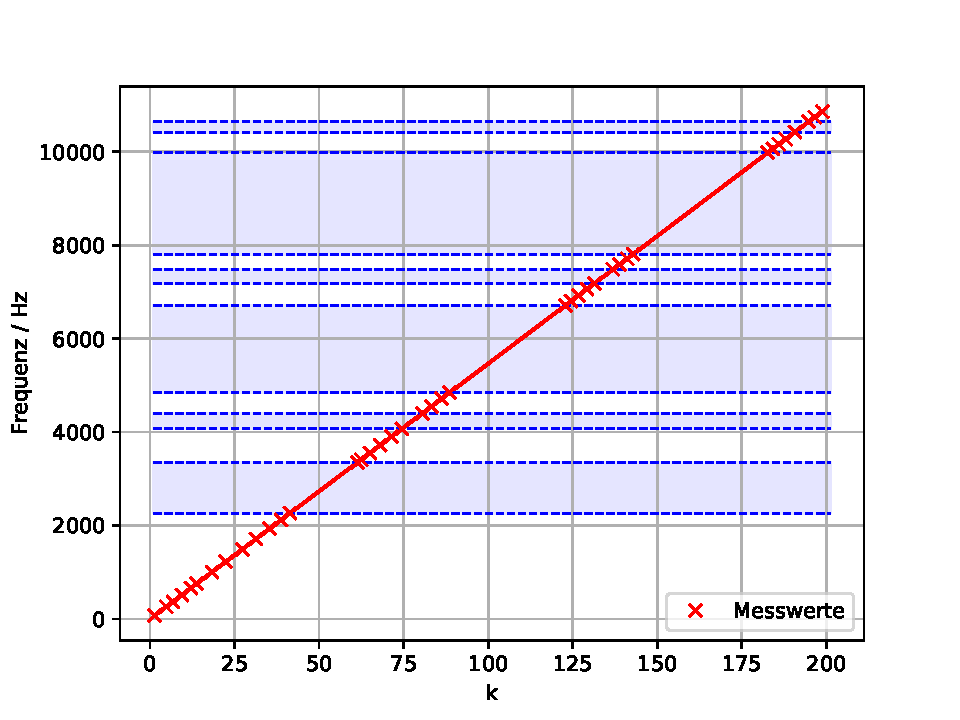
\includegraphics[width=1\textwidth]{A101.pdf}
  \caption{Frequenz der Maxima geplottet gegen k mit makierten Bandlücken}
  \label{fig.Aufgabe101}
\end{figure}
%  \begin{figure}[h!]
%    \centering
%    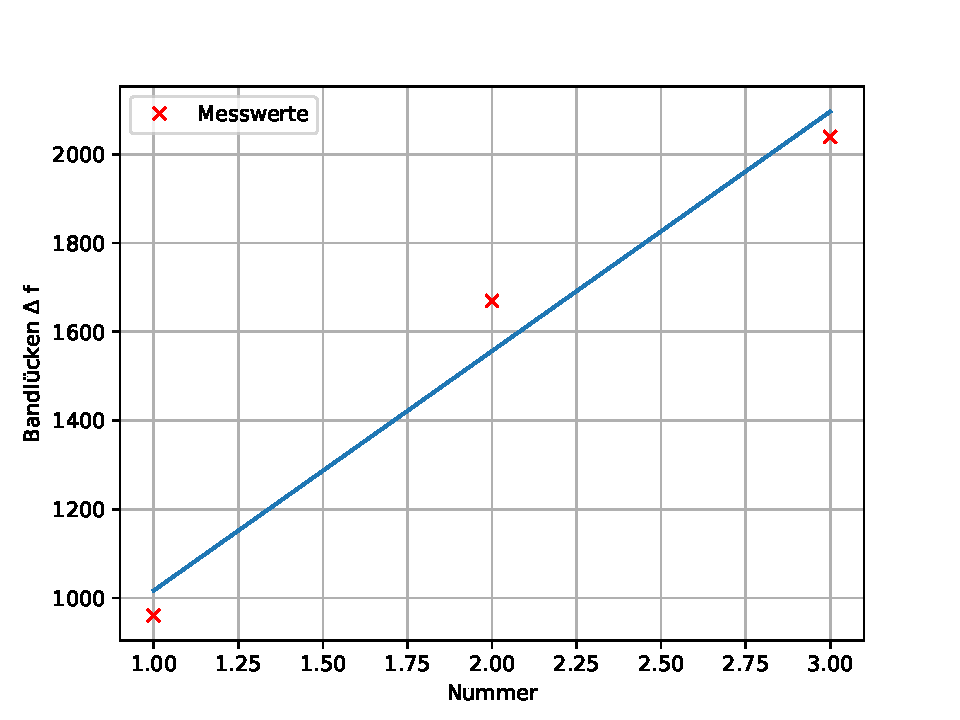
\includegraphics[width=\textwidth]{A10.pdf}
%    \caption{Bandlücken bei alternierenden Blendengrößen}
%    \label{fig.Aufgabe10}
%  \end{figure}
  \FloatBarrier
  %\textbf{\huge{Der Plot hat an der x-Achse keine Einheit}}


\subsection{Aufgabe 11}
In dieser Aufgabe geht es ebenfalls darum, das Verhalten von Bandlücken unter Verwendung von Defekten zu beobachten.
Die Defekte treten hier jedoch nicht wie in der Aufgabe zuvor in Form von der Blendengröße (Bindungsstärke) auf, sondern die Rohrabschnitte (Größe der Einheitszellen) werden verändert.
Für die Messung wird eine alternierende Folge von 50 und $\SI{75}{mm}$ langen Röhren benutzt, welche jeweils mit Blenden vom Durchmesser 16 $\si{mm}$ abgetrennt sind.
Insgesammt werden 10 Rohrabschnitte verwendet.
Auch hier werden zur Veranschaulichung wieder die Frequenzen der Maxima gegen k geplottet.
Anhand der farblich makierten Bandlücken wird deutlich, dass die Defekte einen großen Einfluss auf des Verhalten der Kette haben.
Es lässt sich kein Muster erkennen, nach dem sich die Bandlücken gebildet haben.
%Die Bandlücken werden nummeriert und wie in Abbildung \ref{fig.Aufgabe112} geplottet.
%An der Abbildung ist deutlich zu erkennen das die Größe der Bandlücken nicht mehr wie üblich mit steigender Nummer linear ansteigt.
\begin{figure}[h!]
  \centering
  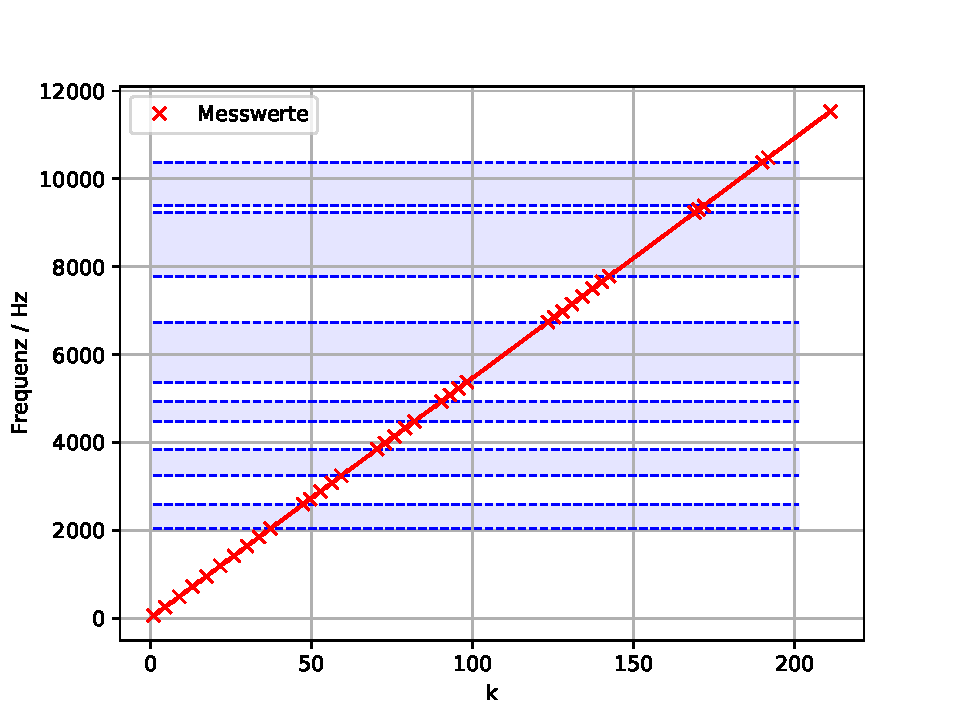
\includegraphics[width=1\textwidth]{A112.pdf}
  \caption{Frequenz der Maxima geplottet gegen k mit makierten Bandlücken}
  \label{fig.Aufgabe111}
\end{figure}
%\begin{figure}[h!]
%  \centering
%  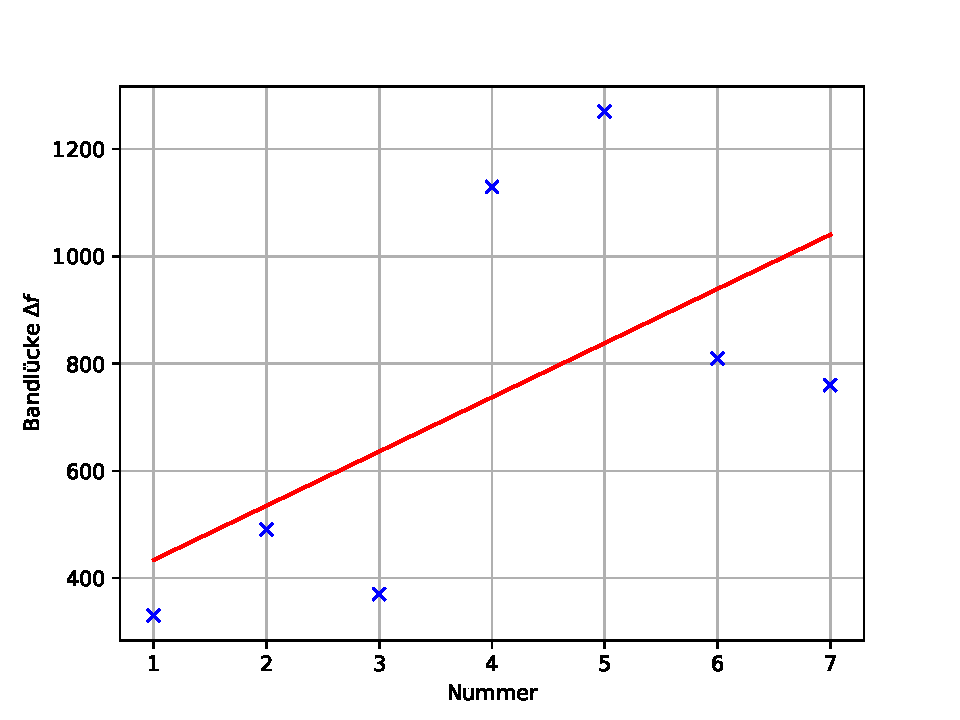
\includegraphics[width=\textwidth]{A11.pdf}
%  \caption{Bandlücken bei alternierenden Rohrlängen}
%  \label{fig.Aufgabe112}
%\end{figure}
\FloatBarrier

\subsection{Aufgabe 12}
Nun werde vereinzelte, unperiodische Defekte in die Kette eingebaut.
Es werden 4 Messungen mit unterschiedlichen Defekten durchgeführt.
Die entstehenden Bandlücken sind in den Abbildungen \ref{fig.Aufgabe12} gut zusehen.
Durch die Defekte entsteht ein Maximum, oder auch ein zusätzlicher Zustand, inerhalb der ersten Bandlücke.

%  \begin{figure}[h!]
%    \centering
%    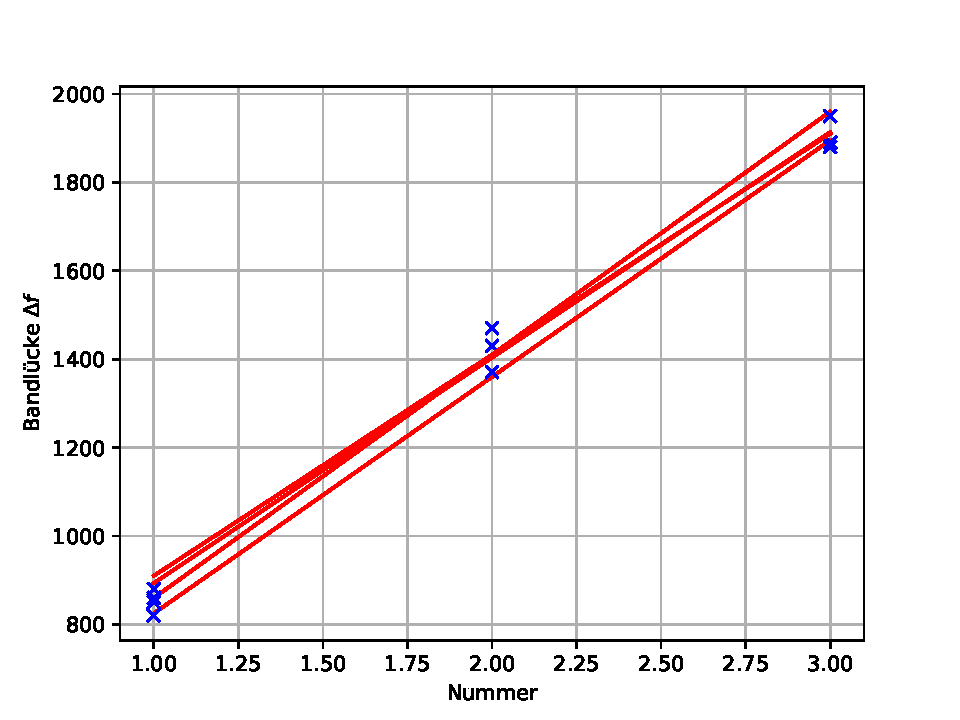
\includegraphics[width=\textwidth]{A12.pdf}
%    \caption{Bandlücken bei alternierenden Rohrlängen}
%    \label{fig.Aufgabe12}
%  \end{figure}
%  \FloatBarrier

  \begin{figure}
   \centering
   \begin{subfigure}{0.48\textwidth}
    \centering
    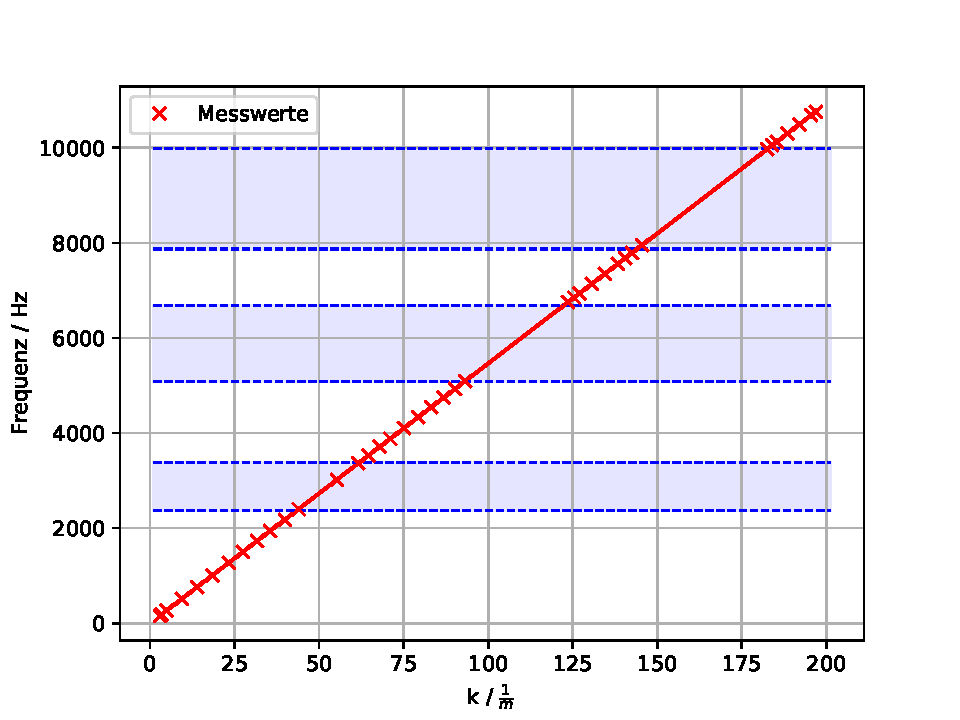
\includegraphics[width=1.1\textwidth]{max.pdf}
    \caption{Defekt an dritter Stelle mit $\SI{12.5}{mm}$}
    \label{fig.Aufgabe121}
   \end{subfigure}
   \begin{subfigure}{0.48\textwidth}
    \centering
    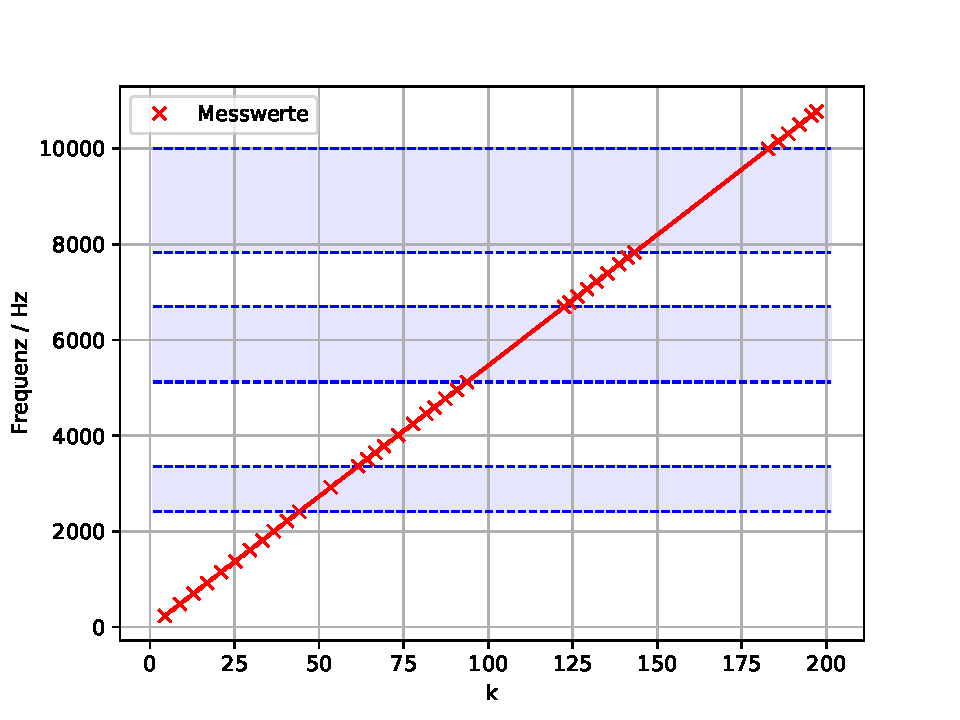
\includegraphics[width=1.1\textwidth]{max2.pdf}
    \caption{Defekt an dritter Stelle mit $\SI{75}{mm}$}
    \label{fig.Aufgabe122}
   \end{subfigure}

   \begin{subfigure}{0.48\textwidth}
    \centering
    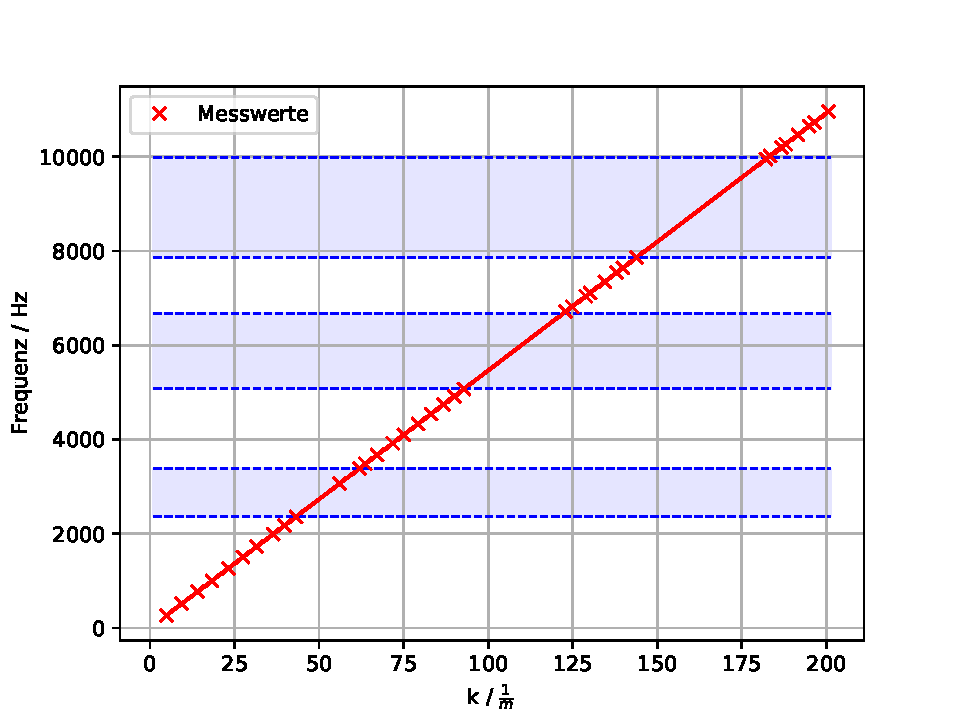
\includegraphics[width=1.1\textwidth]{max3.pdf}
    \caption{Defekt an achter Stelle mit $\SI{12.5}{mm}$}
    \label{fig.Aufgabe123}
   \end{subfigure}
   \begin{subfigure}{0.48\textwidth}
    \centering
    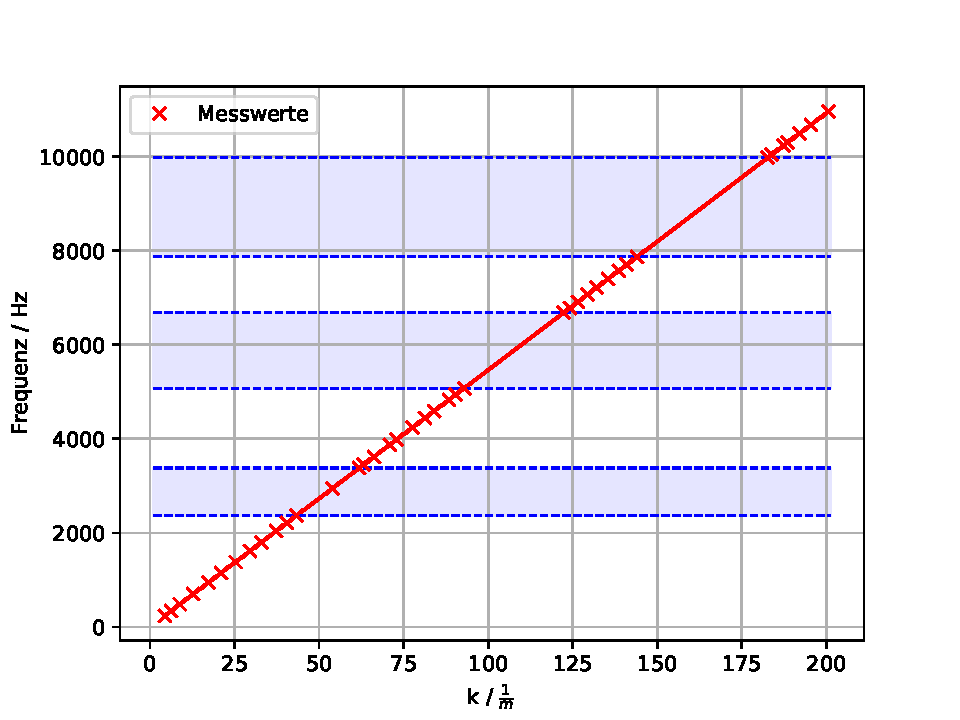
\includegraphics[width=1.1\textwidth]{max4.pdf}
    \caption{Defekt an achter Stelle mit $\SI{75}{mm}$}
    \label{fig.Aufgabe124}
   \end{subfigure}
   \caption{Messung mit einem Rohr der Länge $12 \cdot \SI{50}{mm}$ und einem Blendendurchmesser von $\SI{16}{mm}$ mit Defekten an bestimmten Stellen.}
   \label{fig.Aufgabe12}
  \end{figure}
